
\section{Forráskódolás}
Cél: Tömörítés $\Longrightarrow$ Gyorsabb adatátviteli sebesség

\subsection{Prefix kódok}

$Y^* -$ kódszavak, $X -$ forrásábécé

Egyértelmű dekódolhatóság: Egykávéjöhetmár $\Longrightarrow$ Egy | kávé | jöhet | már

Ez csak akkor működik ha nincs másik szónak ilyen prefixe, egyébként nem tudnánk egyértelműen dekódolni.\\[-2pt]

\begin{definicio}{Mézga Géza} Prefix mentes kód $\Longleftrightarrow$ bináris fa\\[0pt]
\end{definicio}

\subsection{Átlagos kódszóhossz, entrópia}

$p(x) = \mathbf{P}(X = x), x \in X$

p(x) - x forrásbetű valószínűségét jelenti\\[-2pt]


\begin{definicio}{Entrópia}

$$H(X) = \mathbf{E}\Big(-ld(p(X))\Big) = - \sum\limits_{i = 1}^n p(x_i)\cdot ld\left(p(x_i)\right)$$

\small Megjegyzés: $ld(x) = log_2(x)$ innentől \normalsize\\[2pt]
\end{definicio}

\begin{tetel}{Egyértelmű dekódolhatóság feltétele - Kraft egyenlőtlenség}
$$ \sum\limits_{\forall x} 2^{-l(x)} \leq 1$$
\end{tetel}

\begin{definicio}{Mézga Géza} Egy f kód \textbf{Átlagos kódszóhossza}

$$ \mathlarger{\mathbf{L}} = \mathbf{E}|f(X)| = \sum\limits_{i = 1}^n p(x_i)\cdot |f(x_i)| $$
\end{definicio}

\begin{definicio}{Mézga Géza} Egyenletes eloszlással rendelkezőt nem lehet tovább tömöríteni!\\[2pt]
\end{definicio}

\begin{tetel}{MZ/X használhatatlan cuccokat küld}
\textbf{Forráskódolási tétel:}

$$H(X) \leq L$$

\textit{Ha L kisebb mint H(X) akkor nem dekódolható egyértelműen}
\end{tetel}

Biz:\ldots\\[2pt] %TODO

\subsection{Shannon-Fano-kód}

\textbf{Kódkonstrukció}
\begin{itemize}
	\item Adott p(x) $\rightarrow$ $\mathbf{l(x)} = \Gorog{\lceil} ld\left( \dfrac{1}{p(x)} \right) \Gorog{\rceil}$
	\item bináris fa $\rightarrow$ LUT
\end{itemize}
\small PL: Sajat jegyzet 82. oldal \normalsize

\textbf{Tulajdonságok}
\begin{itemize}
	\item A példában is $ \eta = \dfrac{H(X)}{L} \approx 0.8 \Longrightarrow$ Lehet még rajta javítani
	\item Nem egyértelmű a megoldás!(De mindegyik jó)
\end{itemize}

Hogyan tudok optimálisabb kódot készíteni??

\subsection{Blokk kód}

	\begin{enumerate}
		\item $H(X) \leq \lambda^{(k)} \leq H(X) + \dfrac{1}{K}$ \quad ( K blokkok száma )

			 Ha olyan kódot akarunk generálni ami az alsó határt $Z$-vel közelíti $\longrightarrow$

			 $\dfrac{1}{K} \leq Z \cdot H(X) \ \Longrightarrow \left\lceil \dfrac{1}{Z \cdot H(X) } \right\rceil \leq K $

		\item - Komplexitás: $O(2^k)$
	\end{enumerate}

\subsection{Huffman kódolás}



\textbf{Tulajdonságok}
\begin{itemize}
	\item Rekurzív mohó algoritmus
	\item - Tudni kell az eloszlást
	\item - Algoritmus komplexitása
\end{itemize}

%TODO Aritmetikai kódolás könyvből Saját (87, könyv 166)

Gyakorlati kihívások:
\begin{itemize}
	\item p(x) nem adott (Telefonba nem mondják meg :D ) $\rightarrow$ meg kell becsülni
	\item Lehet e p(x) nélkül tömöríteni? $\rightarrow$ Igen
\end{itemize}

\subsection{ Distribution free Compression ( Valószínűség független )}
\begin{enumerate}
	\item LZ78  %TODO Jó példát írni rá
		\begin{itemize}
			\item Szótárat használ,

			\item Minél nagyobb a fájlméret annál jobban konvergál Huffman kódhoz!

			\item PL: 0100010100101000

			\begin{enumerate}
				\item Parsing: 0 1 00 01 010 0101 000

				\item Az így kapott szimbólumokhoz index rendelése binárisan

				\item Táblázat készítése

					\begin{tabular}{|l|c|r||l|}
 					 \hline
 					 Index(bin) & Szimbólum & Output & Output Magyarázat \\ \hline \hline
 					 001 & 0    & (000,0)   & (meg nem volt ilyen, 0 jött) \\  \hline
 					 010 & 1    & (000,1)   & (meg nem volt ilyen, 1 jött)\\  \hline
 					 011 & 00   & (001,0)   & (mar volt 0 a 001 helyen,0 jött)\\  \hline
 					 100 & 01   & (001,1)   & (mar volt 0 a 001 helyen,1 jött)\\  \hline
 					 101 & 010  & (100,0)   & (mar volt 01 a 100 helyen,0 jött)\\  \hline
 					 110 & 0101 & (101,1)   & (mar volt 010 a 101 helyen,1 jött) \\  \hline
 					 111 & 000  & (011,0)   & (mar volt 00 a 011 helyen,0 jött)\\  \hline
					\end{tabular}

			\end{enumerate}


		\end{itemize}
	\item LZ77

		\begin{itemize}
			\item A már előfordult karaktersorozatokat egy hivatkozással és egy hosszal jelzi
			\item Nagyobb hosszt adunk meg a pattern előről indul
			\item Ez is konvergál Huffman kódhoz.
			\item PL: a ac aacab caba

				\begin{enumerate}
					\item Táblázat készítése

					\begin{tabular}{|r|l|c|c|}
 					 \hline
 					 Mar jo & Meg nemjo & Output & Output Magyarázat \\ \hline \hline
 					 - & a acaacabcaba & (0,0,"a") & (Nincs egyezes,,"a" jött) \\ \hline
 					 a & ac aacabcaba & (1,1,"c") & (1 el visszabb, 1 el előre ismétel, c jött) \\ \hline
					aac & aacab caba & (3,4,"b") & (3 al visszabb, 4x ismetel a patternt, b jött) \\ \hline
					aacaacab & caba &  (3,3,"a") & (3 at vissza, 3x ismétel, + a)\\ \hline
					\end{tabular}
				\end{enumerate}
		\end{itemize}

	\item Adaptív Huffman (2 egész számú hatvánnyal csak!)

		\begin{enumerate}
			\item A fát balról jobbra olvasva alúról, egy monoton növekvő sorozatot kell hogy kapjunk!
			\item Az egyes csomópontokban található szám megegyezik a gyerekeikben található számok összegével!

			\item PL Lehet-e ez Adaptív Huffman fa? Miért?
					\begin{center}
						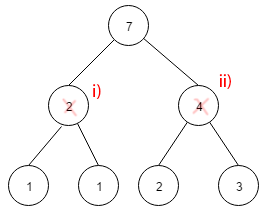
\includegraphics[scale=0.7]{img/AdaptivHuffman}
					\end{center}
				\begin{enumerate}
					\item Ha ott "2" es szerepel akkor egy monoton növekvő sorozatot kapunk: 1,1,2,3,2,4,7

							Helyette 3,4,(5)
					\item Ha ott "4" es szerepel akkor $2+3 \neq 4$, helyette 5
				\end{enumerate}
		\end{enumerate}


		%TODO Diáról kiírni
\end{enumerate}

\subsection{Sokfelhasználós rendszerek kódolási kérdései}

\subsubsection{FDMA - Frequency Division Multiple Access}
	Részletesebben: Rendszer Elmélet nevű tárgyból.

	\begin{center}
		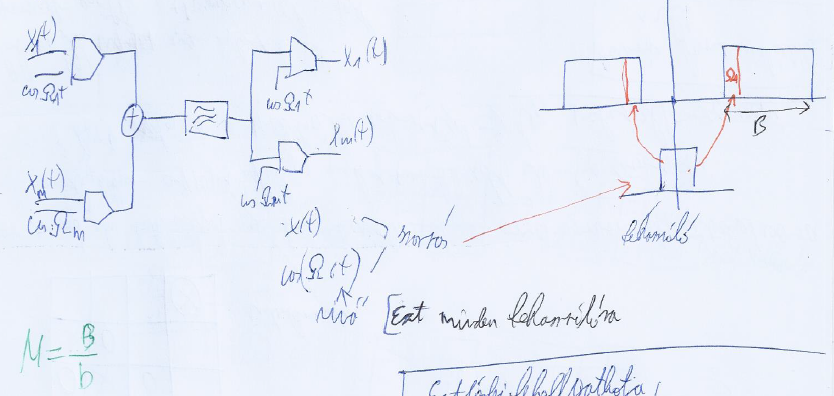
\includegraphics[scale=0.8]{img/FDMA}
	\end{center}

\subsubsection{TDMA - Time Division Multiple Access}

	Beszéd típusú kommunikációra ez is tökéletes.

\subsubsection{CDMA - Code Division Multiple Access}
	Ezt használják a telefonok

	\begin{enumerate}
		\item \textbf{Frequency Hopping}

		\begin{itemize}

			\item	PL: Bluetooth, mert visszaverődik és nehéz detektálni

			\item	Küldés:
				\begin{center}
					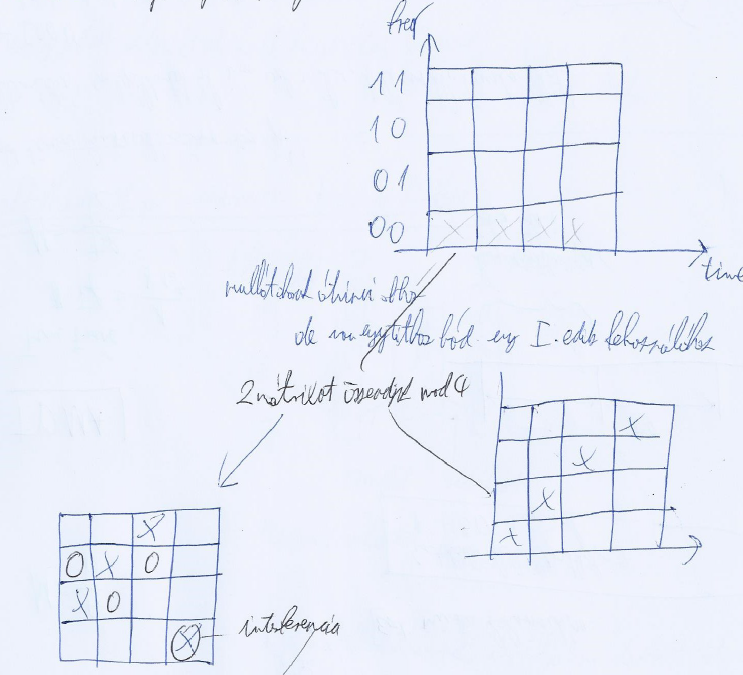
\includegraphics[scale=0.8]{img/CDMA1}
				\end{center}
			\item	Fogadás:
				\begin{center}
					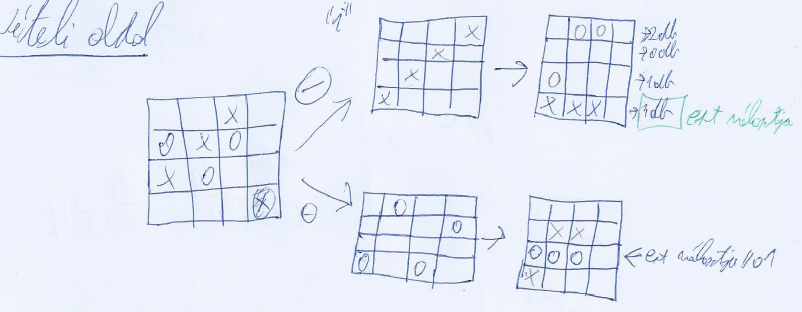
\includegraphics[scale=0.8]{img/CDMA2}
				\end{center}
		\end{itemize}

		\item \textbf{Direct Sequence}

			\begin{itemize}
				\item PL: \textbf{b3G}

				\item Van M db felhasználó aki közös forrást használ.

				\item A kódszó vektoroknak Ortogonálisnak kell lenniűk, különben mindenki megkapja a másik üzenetét is ( \textit{interferncia} )

				\begin{center}
					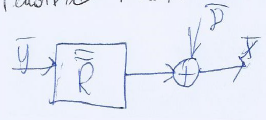
\includegraphics[scale=0.8]{img/CDMA3}

					$\nu = Zaj$
				\end{center}

				\item $R_{i,j} = \dfrac{1}{N} \overline{C}^{(i)T} \cdot \overline{C}^{(j)}$

				ahol N = kódszó hossz, és a 2 vektor szorzásából egy konstans lesz


			\end{itemize}
		\begin{definicio}{Mézga Géza} \textbf{Walsh-hadamart algoritmus}
			\begin{center}
				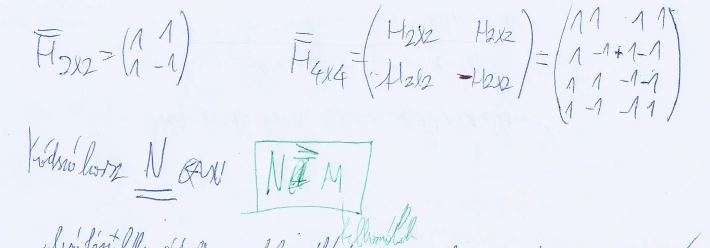
\includegraphics[scale=0.8]{img/CDMA4}
			\end{center}
			Így ortogonális. Kissebb számítás igényű mint az előtte lévő, de kevesebb embert tud kiszolgálni
    \end{definicio}

	\end{enumerate}
